\documentclass[12pt]{article}
%% arXiv paper template by Flip Tanedo
%% last updated: Dec 2016



%%%%%%%%%%%%%%%%%%%%%%%%%%%%%
%%%  THE USUAL PACKAGES  %%%%
%%%%%%%%%%%%%%%%%%%%%%%%%%%%%

\usepackage{amsmath}
\usepackage{amssymb}
\usepackage{amsfonts}
\usepackage{graphicx}
\usepackage{xcolor}
\usepackage{nopageno}
\usepackage{enumerate}
\usepackage{parskip}
\usepackage{framed}
%\usepackage{bbm} 
\usepackage[normalem]{ulem}


\renewcommand{\thesection}{}
\renewcommand{\thesubsection}{\arabic{subsection}}

%%%%%%%%%%%%%%%%%%%%%%%%%%%%%%%%%%%%%%%%%%%%%%%
%%%  PAGE FORMATTING and (RE)NEW COMMANDS  %%%%
%%%%%%%%%%%%%%%%%%%%%%%%%%%%%%%%%%%%%%%%%%%%%%%

\usepackage[margin=2cm]{geometry}   % reasonable margins

\graphicspath{{figures/}}	        % set directory for figures

% for capitalized things
\newcommand{\acro}[1]{\textsc{\MakeLowercase{#1}}}    

%\numberwithin{equation}{section}    % set equation numbering
\renewcommand{\tilde}{\widetilde}   % tilde over characters
%\renewcommand{\vec}[1]{\mathbf{#1}} % vectors are boldface

\newcommand{\dbar}{d\mkern-6mu\mathchar'26}    % for d/2pi
\newcommand{\ket}[1]{\left|#1\right\rangle}    % <#1|
\newcommand{\bra}[1]{\left\langle#1\right|}    % |#1>
\newcommand{\Xmark}{\text{\sffamily X}}        % cross out

\let\olditemize\itemize
\renewcommand{\itemize}{
  \olditemize
  \setlength{\itemsep}{1pt}
  \setlength{\parskip}{0pt}
  \setlength{\parsep}{0pt}
}


% Commands for temporary comments
\newcommand{\comment}[2]{\textcolor{red}{[\textbf{#1} #2]}}
\newcommand{\flip}[1]{{\color{red} [\textbf{Flip}: {#1}]}}
\newcommand{\email}[1]{\texttt{\href{mailto:#1}{#1}}}

\newenvironment{institutions}[1][2em]{\begin{list}{}{\setlength\leftmargin{#1}\setlength\rightmargin{#1}}\item[]}{\end{list}}


\usepackage{fancyhdr}		% to put preprint number



% Commands for listings package
%\usepackage{listings}      % \begin{lstlisting}, for code
%
% \lstset{basicstyle=\ttfamily\footnotesize,breaklines=true}
%    sets style to small true-type



%%%%%%%%%%%%%%%%%%%
%%%  HYPERREF  %%%%
%%%%%%%%%%%%%%%%%%%

%% This package has to be at the end; can lead to conflicts
\usepackage{microtype}
\usepackage[
	colorlinks=true,
	citecolor=black,
	linkcolor=black,
	urlcolor=green!50!black,
	hypertexnames=false]{hyperref}





\begin{document}


\begin{center}

    {\Large \textsc{Long HW 4}:
    \textbf{Electroweak, Action}}
    
\end{center}

\vskip .4cm

\noindent
\begin{tabular*}{\textwidth}{rl}
	\textsc{Course:}& Physics 165, \emph{Introduction to Particle Physics} (2018)
	\\
	\textsc{Instructor:}& Prof. Flip Tanedo (\email{flip.tanedo@ucr.edu})
	\\
	\textsc{Due by:}& \textbf{Tuesday}, February 6 \flip{You can turn it in Thursday}
\end{tabular*}

\noindent
This is the main weekly homework set. Unless otherwise stated, give all responses in natural units where $c = \hbar = 1$ and energy is measured in electron volts (usually MeV or GeV). 

\flip{Corrections: 2/5. Thanks to Tommy W.\ and Adam G.}

\subsection{Flavor in the electroweak theory of leptons}

Consider the `unbroken, leptonic electroweak theory' that we studied this week in lecture. The particle content is described in short homework 4. In this problem we will generalize to the case of two \textbf{generations} of fermions. 

\subsubsection{Flavor symmetry}

Introduce a new symmetry to the theory: SU(2) \textbf{flavor}. This is a \textbf{global symmetry}, which means it doesn't come with a spin-1 gauge boson. The structure of this symmetry is the same as SU(2) weak but is totally independent. To make life simpler still, we will only need to think about the fundamental representation. A flavor doublet (fundamental) will have an upper index $i$, the anti-doublet (anti-fundamental) will have a lower index $j$:
\begin{align}
	(\text{flavor doublet})^i &&
	\left[(\text{flavor doublet})^\dag\right]_j \ .
\end{align}
The only tensor that we'll need is $\delta^i_j$. 

Now assume that the lepton doublet $L$ and the positron $\bar E$ are flavor fundamentals. Including spin, SU(2) weak, and SU(2) flavor these particles have quantum numbers:
\begin{align}
	L^{\alpha a i} && \bar E^{\alpha j} \ .
\end{align}
Identify the particles as follows: \flip{Corrected $i$ and $a$ confusion}
\begin{align}
	L^{\alpha(a=1)(i=1)} &= \nu_{eL}^\alpha
	&
	L^{\alpha(a=2)(i=1)} &= e_L^\alpha
	&
	L^{\alpha(a=1)(i=2)} &= \nu_{\mu L}^\alpha
	&
	L^{\alpha(a=2)(i=2)} &= \mu^\alpha
\end{align}
And
\begin{align}
	\bar E^{\alpha(j=1)} &= \left(e_R^\dag\right)^\alpha
	&
	\bar E^{\alpha(j=2)} &= \left(\mu_R^\dag\right)^\alpha \ .
\end{align}
Draw all of the three-particle interactions between $W^\pm_\mu$, $W^3_\mu$, $B_\mu$, and each of the component particles above. 

\textsc{Remark}: You will find that these are just two copies of the same rules you derived in the short homework (and that we did in class). 

\subsubsection{Kinematics Review}

So far all of our particles are massless. Argue that it is \emph{kinematically} impossible to have $\mu \to e B$ or $\mu \to e W^3$, whether or not the underlying \emph{dynamics} allows it.

\subsubsection{Flavor symmetry at work}

Even though it is \emph{kinematically} impossible to have $\mu \to e B$ or $\mu \to e W^3$, maybe it is \textbf{dynamically} possible. Our dynamics (Feynman rules) are determined by symmetries: the symmetries tell us whether or not we can draw a Feynman rule.

Is it possible for the gauge bosons to connect an electron-flavored ($i=1$) fermion with a muon-flavored ($i=2$) fermion? In no more than a few sentences, argue why or why not. Is it possible to draw a diagram for $\mu \to e \gamma$ using only the fermions and spin-1 bosons?


\subsubsection{SU(2)$_L\times$SU(2)$_E$}

Actually, it turns out that there's an \emph{larger} symmetry in the part of the theory we've looked at so far. Argue that the Feynman rules in 1.1 are symmetric under \emph{independent} rotations of $L$ and $\bar E$ in flavor space. This means I could do a flavor rotation on `only the doublets' and the theory would still be symmetric. Why is this so?

This means we could have written indices this way:
\begin{align}
	L^{\alpha a i} 
	&&
	(L^\dag)^{\dot\alpha}_{a i}
	&&
	\bar E^{\alpha j'} 
	&&
	(\bar E^\dag)^{\dot\alpha}_{j'} 
	\ ,
\end{align}
where the primed and un-primed $i,j$ indices have nothing to do with each other and cannot be contracted. 

Because there are two independent rotations we can do, we say that the symmetry group is the product of the two symmetries, SU(2)$_L\times$SU(2)$_E$.

\subsubsection{SU(2)$_L\times$SU(2)$_E$ vs. Yukawa}

Recall the three-particle interactions between a Higgs and the $L$, $\bar E$ fermions from short homework 4. When we promote the fermions to transform under the full SU(2)$_L\times$SU(2)$_E$ flavor symmetry---$L$ under SU(2)$_L$ and $\bar E$ under SU(2)$_E$---are these terms still valid?

\textsc{Remark:} Well. It looks like the symmetries of theory prohibit the Yukawa interactions. 

\subsubsection{The Higgs sector at work: spurions}

The theory we want to build has Yukawa interactions. This means that SU(2)$_L\times$SU(2)$_E$ is not a true symmetry of the theory we want. However, it turns out that it's still useful as an \emph{approximate} symmetry\footnote{You should be thinking to things: (1) What does this mean? (2) It probably means something with a Taylor expansion.}. One way to account for this approximate-ness is to introduce an \textbf{order parameter} for how bad the symmetry is. 

`Order parameter' is a phrase borrowed from condensed matter that's actually not technically the best term. Particle theorists use the term \textbf{spurion} for a `fake' invariant tensor. It's an object that has indices of a symmetry, but that isn't actually invariant and doesn't actually transform. The symmetry is broken, but it's broken in a specific, parameterized way. 

Here's how it works for the SU(2)$_L\times$SU(2)$_E$ flavor symmetry. Introduce a spurion $y_{ij'}$ called a \textbf{Yukawa coupling}. This connects one SU(2)$_L$ index to an SU(2)$_E$ index. You can use $y_{ij'}$ to ``soak up'' indices to write down Feynman rules.

Write down the three-particle Feynman rules for the Higgs an two fermions using the $y_{ij'}$. 

\textsc{Remark}: Why is this useful? \emph{Most} of the theory respects SU(2)$_L\times$SU(2)$_E$ symmetry. We saw that this leads to certain processes being prohibited. Now there's one piece of the theory that \emph{doesn't} respect SU(2)$_L\times$SU(2)$_E$. That means that any process that violates the big symmetry must be proportional to Yukawa coupling. If the Yukawa coupling is small, then the rate for that process is small. 


\subsubsection{SU(2)$_L\times$SU(2)$_E$ Breaking}

\flip{2/5: Fixed indices, removed last question}

Assume that $y_{ij'}$ is an arbitrary $2\times 2$ complex matrix. By performing SU(2)$_L\times$SU(2)$_E$ rotation, the Yukawa coupling transforms as:
\begin{align}
	L^i y_{ij'}\bar E^{j'} 
	\to 
	L^i (U_L)^k_{\phantom k i} y_{k\ell'} (U_E)^{\ell'}_{\phantom{\ell'} j'} E^{j'} \ ,
\end{align}
in other words, 
\begin{align}
	y_{ij'} \to (U_L)^k_{\phantom k i} y_{k\ell'} (U_E)^{\ell'}_{\phantom{\ell'} j'} \ .
\end{align}
This boils down to rotating on the left and on the right by two arbitrary matrices. Answer the following questions:
\begin{itemize}
	\item In general, can $y_{ij'}$ be diagonalized by this transformation?
	\item In general, is $y_{ij'}$ proportional to the identity matrix?
	\item \flip{Forget this question}. \textcolor{red}{\sout{Argue that there is some leftover U(1) charge that is conserved. That is, show that there is some SU(2)$_L\times$SU(2)$_E$ rotation that preserves the diagonalized form of $y_{ij'}$. (\textsc{Hint}: what Abelian \emph{flavor} symmetries are available?)}}
\end{itemize}

\textcolor{red}{\sout{Do the leftover symmetries of the dynamics permit $\mu\to e B$ or $\mu \to e W^3$?}}

\textsc{Remark}: We'll wait until next time to show that this can actually happen. First we need to see how fermion masses work out in this theory.


\subsection{Gaussian Integrals}

The last theoretical step that we need to develop is an understanding of the \textbf{action}, $S$. Gaussian integrals are one way to build the foundations for this, even though they look like they have nothing to do with anything. \flip{2/5 hint: P231 lecture notes posted} Feel free to refer to the Physics 231 (Fall 2017) lecture notes\footnote{\url{https://github.com/Tanedo/Physics165-2018/blob/master/Homework/P165_2018_4b_hint.pdf}} on this topic, where the key steps are outlined. Write them up yourself and understand what each step is doing.

\subsubsection{One dimensional Gaussian integrals}

\begin{itemize}
	\item Show that $\int_{-\infty}^\infty dx\; e^{-\frac 12 x^2} = \sqrt{2\pi}$.
	\item Use a simple rescaling argument to evaluate $\int_{-\infty}^\infty dx\; e^{-\frac a2 x^2}$. \\(You could have guessed from dimensional analysis.)
	\item Complete the square to evaluate $\int_{-\infty}^\infty dx\; e^{-\frac a2 x^2 + Jx}$.
\end{itemize}

\subsubsection{$N$ dimensional integrals}

Now consider the $N$-dimensional Gaussian integral in ordinary Euclidean space:
\begin{align}
	\int_{-\infty}^\infty
	dx_1 \, dx_2 \, \cdots \, dx_N \;
	e^{-\frac 12 x_i  A^i_{\phantom{i}j} x^j  + J_i x^i} \ .
\end{align}
Change variables so that $y^i = R^i_{\phantom{i}j}  x^j$ and $J'_i \equiv J_j(R^{-1})^j_{\phantom{j}i}$. Here $R$ is the rotation that diagonalizes $A$. In other words, this change of variables converts the above integral to
\begin{align}
	\int_{-\infty}^\infty
	dy_1 \, dy_2 \, \cdots \, dy_N \;
	e^{-\frac 12 y_i \hat{A}^i_{\phantom{i}j}  y^j  + J'_i y^i} \ ,
\end{align}
where $\hat A = \text{diag}(\hat a_1, \hat a_2, \cdots, \hat a_N)$. Show that the result of this integral is:
\begin{align}
	\sqrt{\frac{(2\pi)^N}{\text{det }A}} e^{\frac 12 J_i (A^{-1})^i_{\phantom{i}j} J^j} \ .
\end{align}
\flip{2/5 Hint: the indices refer to space. The metric for lowering/raising is $\delta_{ij}$ or $\delta^{ij}$. Equivalently, you can treat all indices as lower.}

\subsubsection{1D Expectation Values}

Define
\begin{align}
	\langle x^n \rangle = \int_{\infty}^\infty dx \; x^n \; e^{-\frac 12 ax^2} \ .
\end{align}

Prove the useful fact:
\begin{align}
	\langle x^{2n} \rangle &= \left(-2\frac{d}{da}\right)^n Z
	& 
	Z &= \int_{-\infty}^\infty dx\; p(x) 
	&
	p(x) &=  e^{-\frac 12 ax^2}\ .
\end{align}


\begin{itemize}
	\item Show that $\langle x\rangle = 0$ \ .
	\item Show that $\langle x^2\rangle = \sqrt{2\pi} a^{-3/2}$ \ .
\end{itemize}

\textsc{Remark}: You should feel confident that this is really just asking for features of some \textbf{distribution}, $p(x)$; up to some normalization. Then $\langle x \rangle$ is the mean of the distribution and $\langle x^2 \rangle$ is the standard deviation (maybe squared, maybe with some prefactors... I don't know, do I look like a statistics reference?).  

\subsubsection{$N$ dimensional correlation functions}

Now let's get to the main part. Suppose you have some distribution over $N$ variables, $q_i$. We're changing notation for a good reason. The analog of $Z$ is
\begin{align}
	Z & = \int_{-\infty}^\infty dq_1\, dq_2\, \cdots dq_N \;
	e^{-\frac 12 q_i A^i_{\phantom{i}j} q^j}
	e^{J_i q^i}
	= 
	\sqrt{\frac{(2\pi)^N}{\text{det }A}} e^{\frac 12 J_i (A^{-1})^i_{\phantom{i}j} J^j} \ .
\end{align}
If you want to call this thing a \textbf{partition function}, then you're doing statistical mechanics. If you also take $N\to \infty$, then you're doing statistical field theory. The only difference between `statistical' and `quantum' is whether the randomness is thermal or quantum.

Define
\begin{align}
	\langle q_i q_j \rangle = \frac{1}{Z}  
	\int_{-\infty}^\infty dq_1\, dq_2\, \cdots dq_N \;
	\left(q_i q_j\right)
	\;
	e^{-\frac 12 q_i A^i_{\phantom{i}j} q^j}
	e^{J_i q^i}
\end{align}
Show that
\begin{align}
	\langle q_i q_j \rangle = A^{-1}_{ij} \ .
\end{align}
\textsc{Hint}: I suggest taking derivatives of $Z$ with respect to $d/dJ^i$ and $d/dJ^j$. 

\flip{2/5, additional hint:} It may be useful to consider the following:
\begin{align}
	\frac{\partial}{\partial J^i} J^k &= \delta^k_i 
	&
	\frac{\partial}{\partial J^i} J_k &= 
	\frac{\partial}{\partial J^i}
	 \delta_{k\ell}J^\ell
	= \delta_{k\ell} \delta^\ell_i 
	= \delta_{ki} \ .
\end{align}
Or you can just lower all indices. 

\flip{2/5, additional remark:} In case you're worried about the order of indices, you can rest assured that $A$ and $A^{-1}$ are symmetric matrices.

\textsc{Remark}: So what? What the heck is this all good for? This correlation function is related to what fancy people call a \textbf{Green's function}, and what everyone calls a \textbf{propagator}. Imagine that spacetime is a big lattice. Each lattice point can be labelled, $i=1,2,3,\cdots$. 
%
Our \textbf{amplitudes} are asking: if I see a particle $q$ at lattice point $i$, what is the \emph{correlation} in my theory of seeing a particle $q$ at lattice point $j$ (where this lattice point is presumably forward in time and somewhere else in space).  Think of $q_i$ as a number that is something like the ``wavefunction'' for seeing a particle at $i$. In fact, it's the value of the quantum field at lattice point $i$. Given a theory---which is somehow encoded in the matrix $A$---we want to know how quantum wobbles at $i$ are propagated to another point $j$.

\textsc{Remark}: In the continuum version of the theory, $i$ and $j$ are replaced with spacetime positions $x$ and $y$. So we talk the fields at $x$ and $y$, $q(x)$ and $q(y)$ respectively. 

\textsc{Remark}: This is secretly the mathematical underpinning of the \textbf{path integral formalism} of quantum field theory. The only thing to identify is
\begin{align}
	e^{-\frac 12 q_i A^i_{\phantom{i}j} q^j} \to e^{iS_\text{quadratic}} \ .
\end{align}


\subsection{Video watching assignment}

Watch the PBS Space Time video ``Feynman's Infinite Quantum Paths\footnote{\url{https://youtu.be/vSFRN-ymfgE}}.'' 

Here are three paths (\textsc{i, ii, iii}) between two states. In the sketch on the right, the space of paths has been projected onto the one-dimensional $x$-axis and the action $S$ is shown on the $y$-axis. The action for the three paths are marked.
\begin{center}
	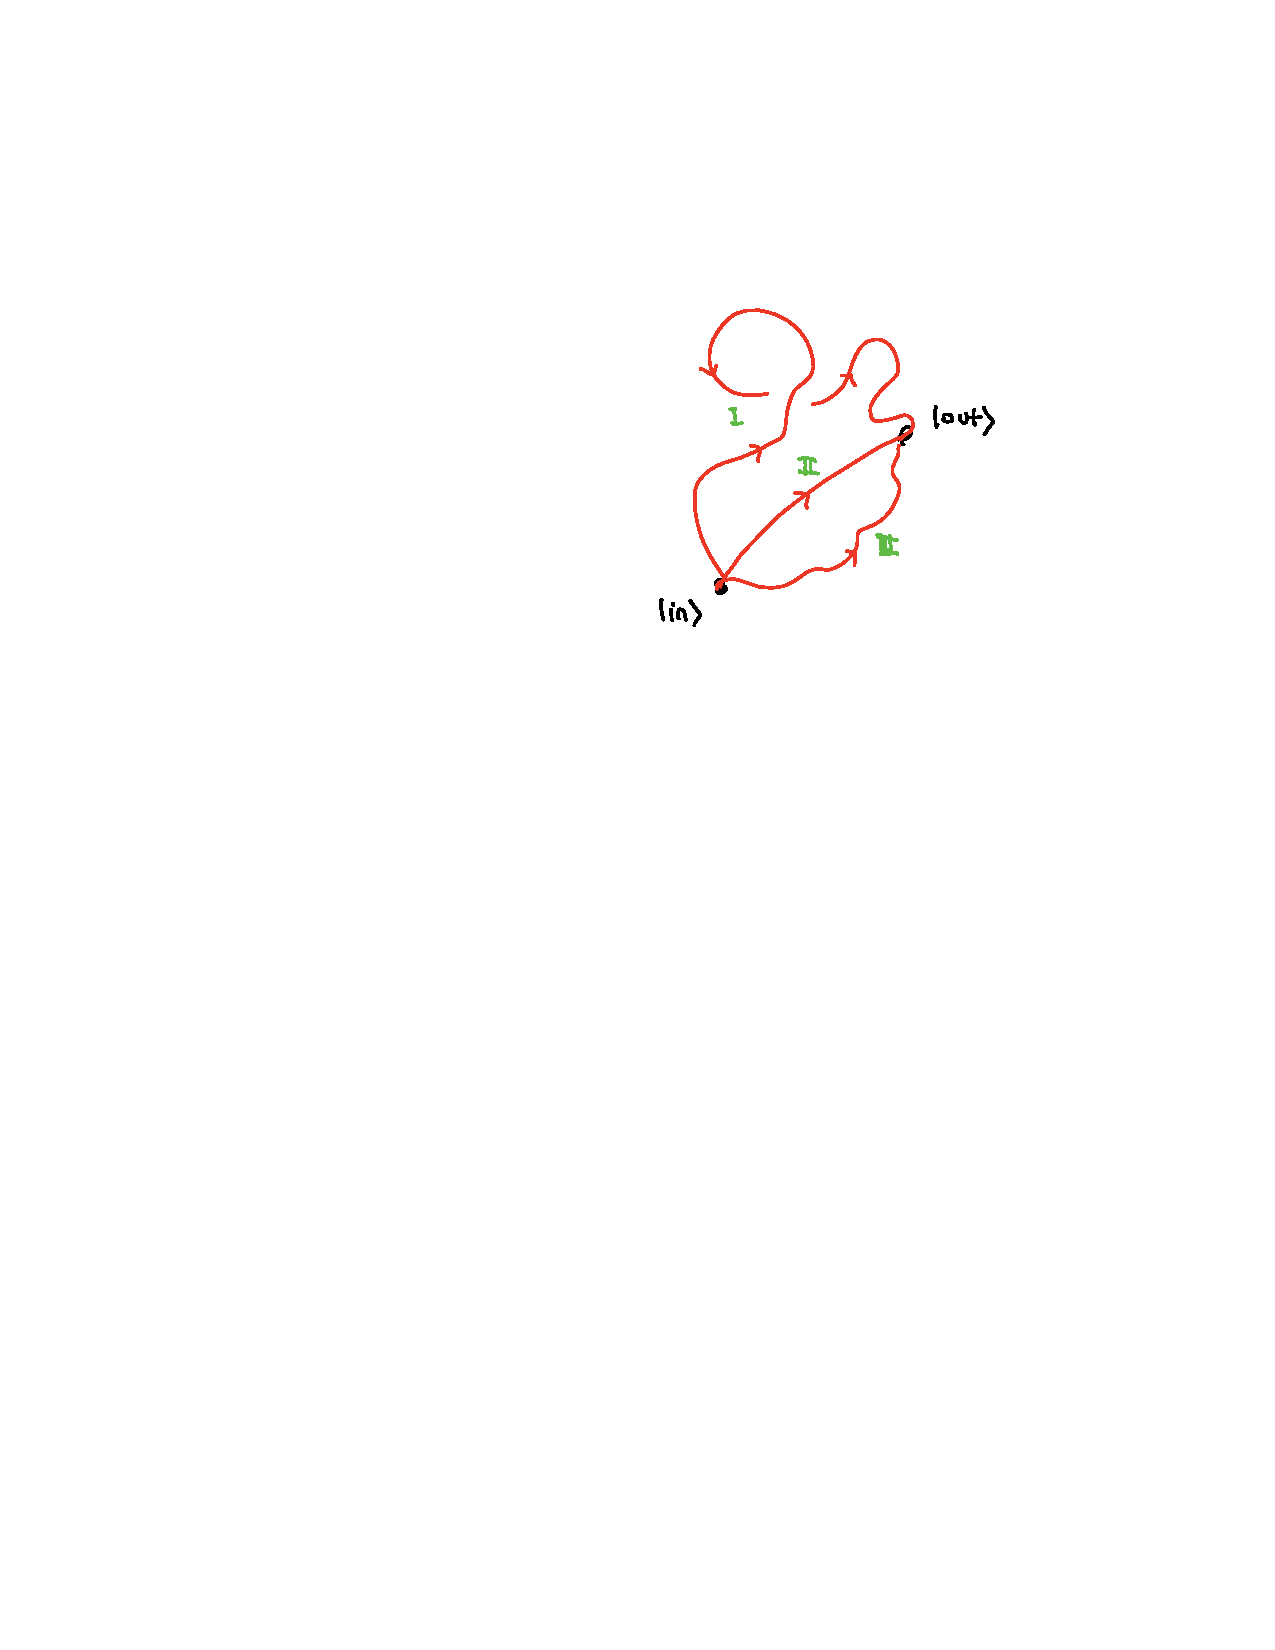
\includegraphics[width=.3\textwidth]{HW4bb}
	\qquad\qquad
	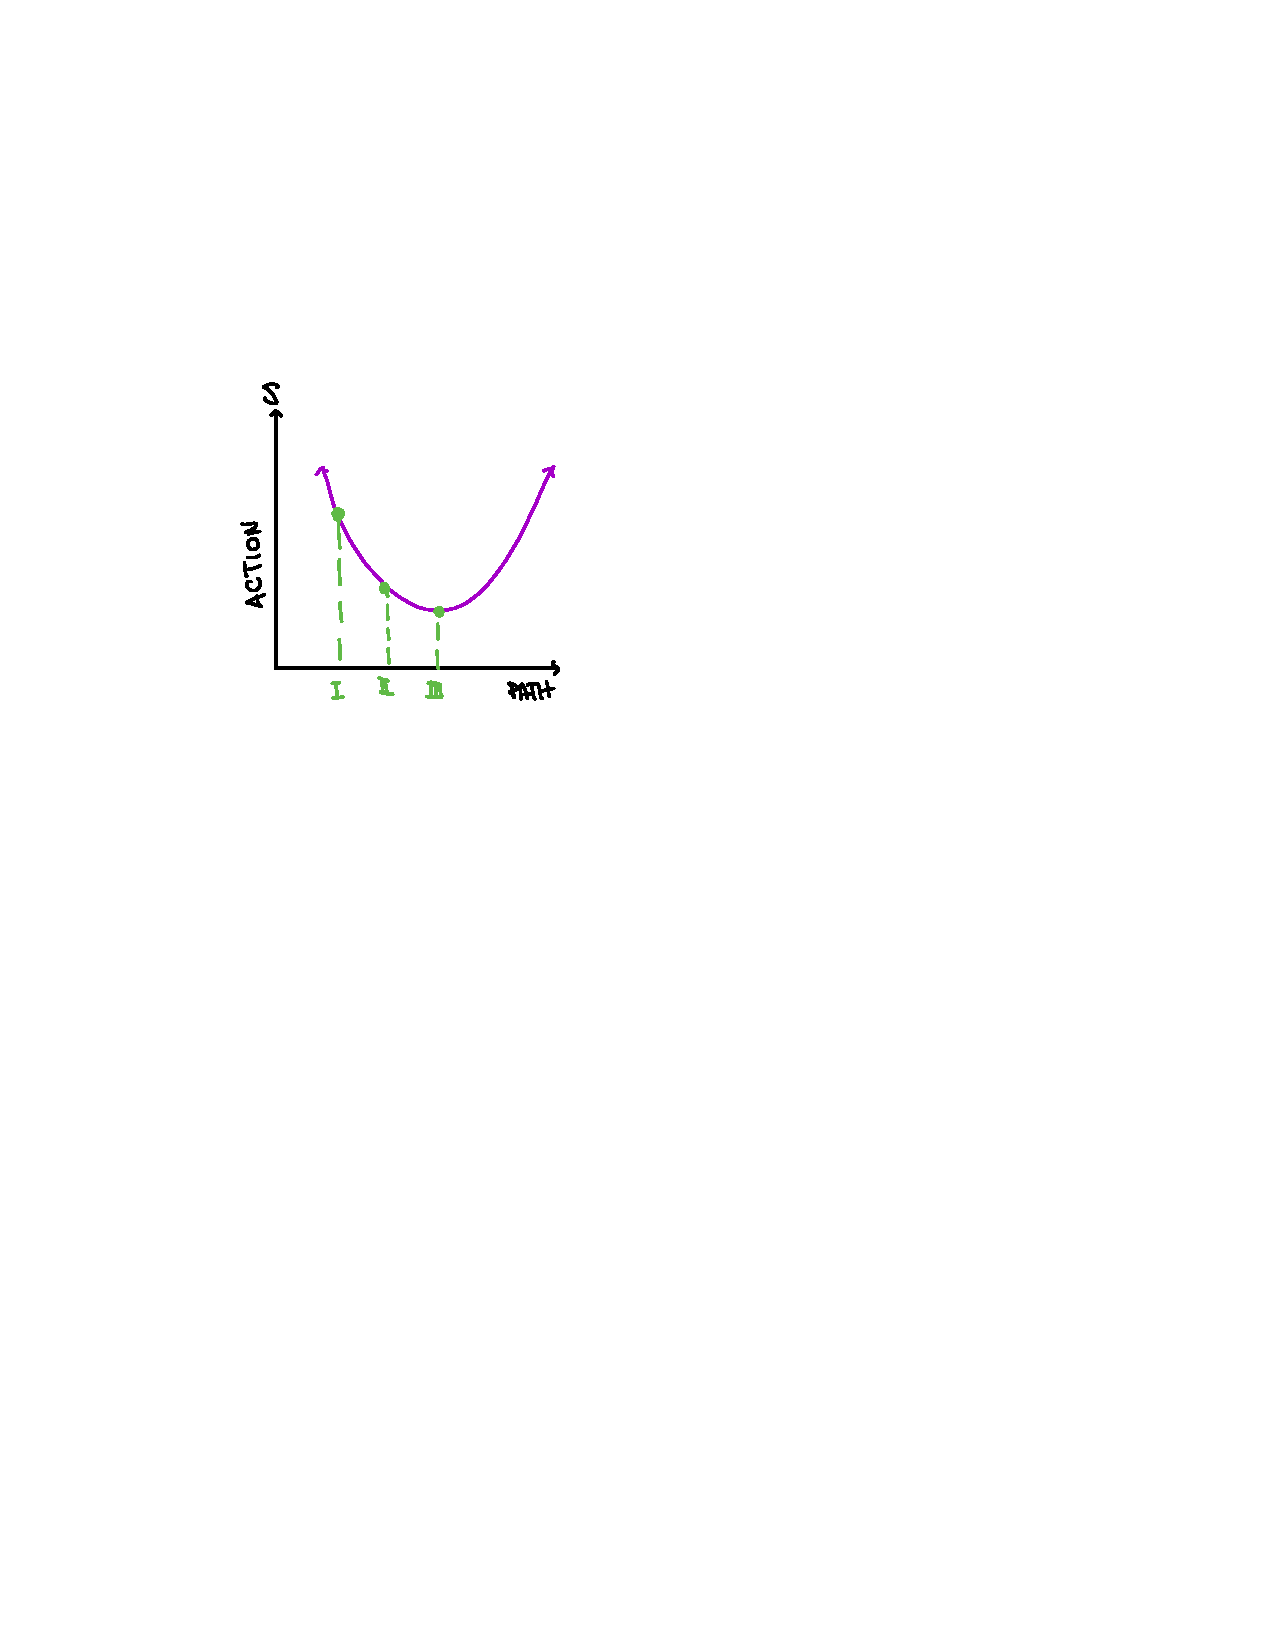
\includegraphics[width=.3\textwidth]{HW4bbb}
\end{center}

In the path integral formalism each path weighted by a complex number, $e^{iS}$. If we sum together a bunch of these paths, we get a phasor diagram:
\begin{center}
	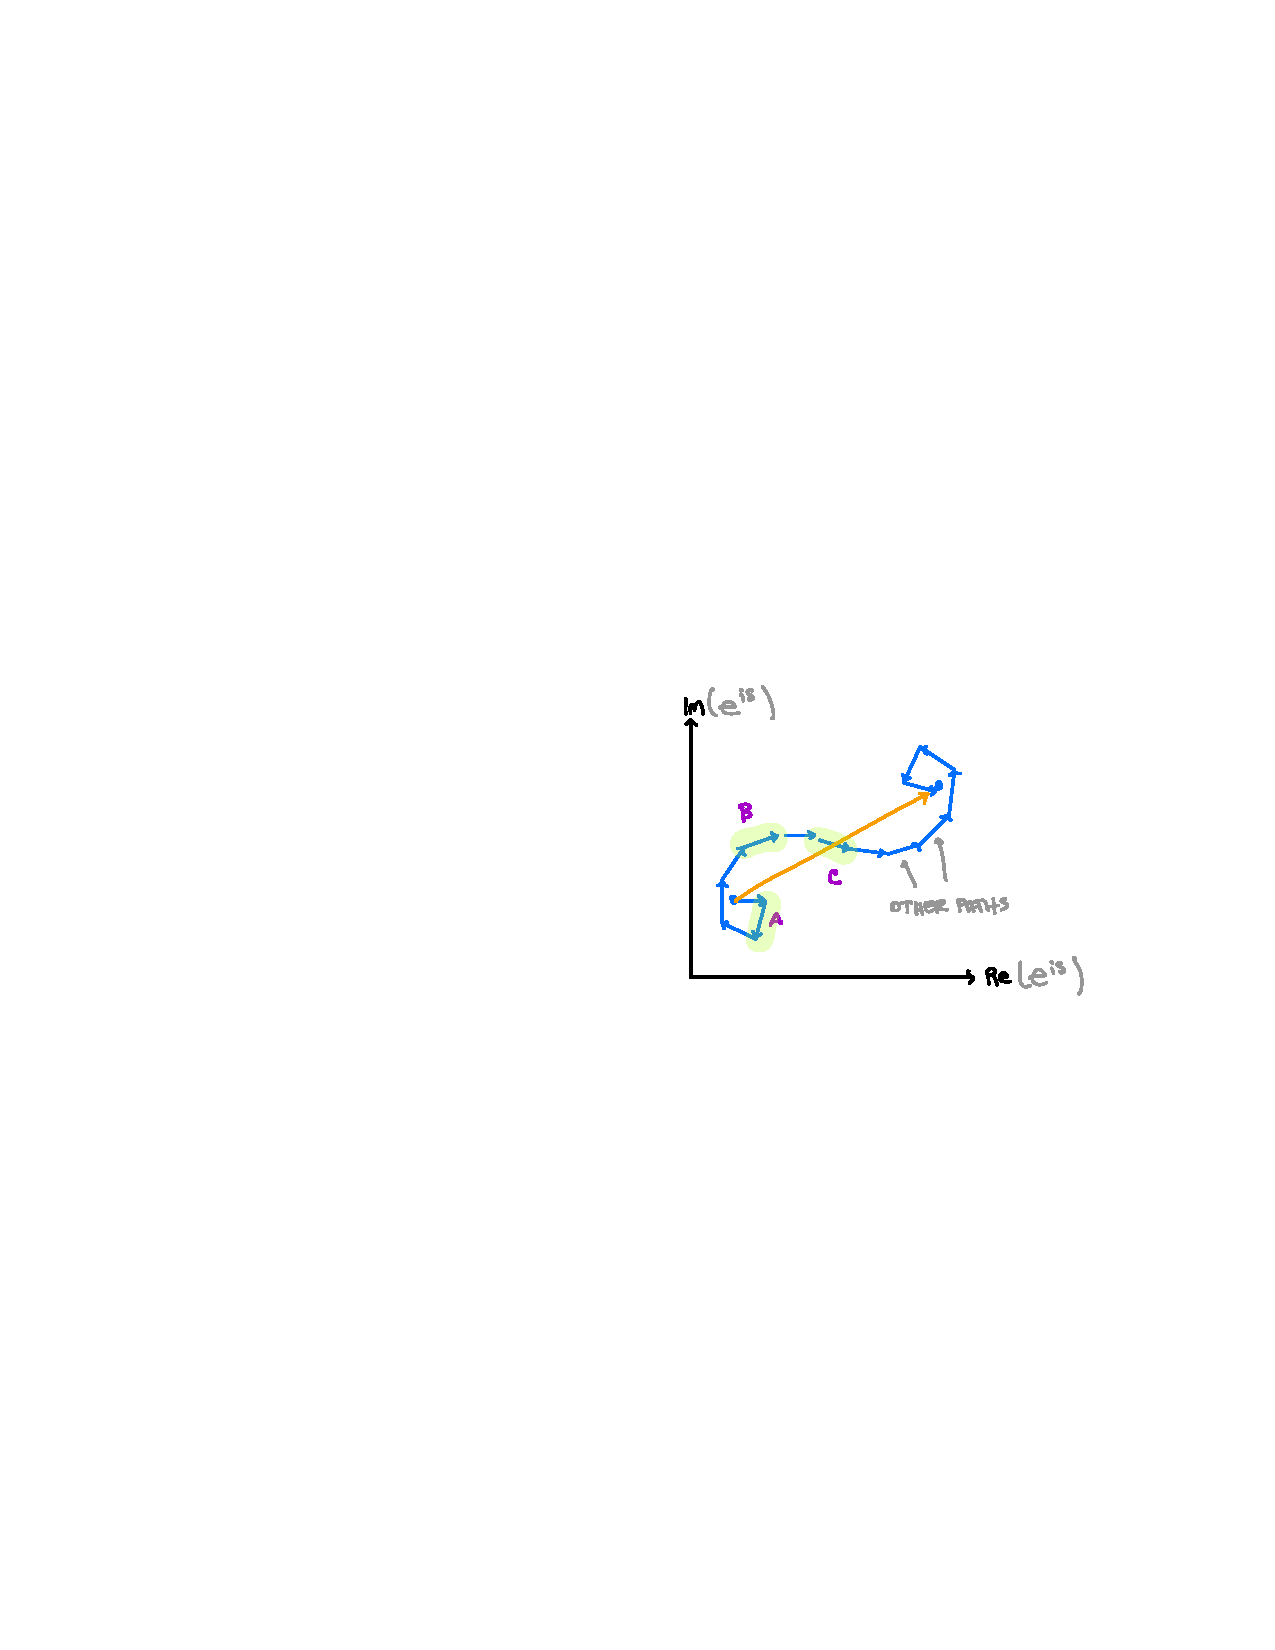
\includegraphics[width=.5\textwidth]{HW4b}
\end{center}
Here the sum in the complex plane is shown graphically: each term in the sum is a unit vector whose base is attached to the endpoint of the previous term. Three terms in the sum are highlighted, $A$, $B$, $C$.

Which of the highlighted terms in the phasor diagram are identified with \textsc{i, ii, iii}? Why is it that we say paths close to the minimum of the action `dominate' the path integral? Why do `crazy' paths, with large values of action, not contribute much?



\textsc{Remark}: This video misspells `Lagrangian.' Feynman presented this approach to path integrals and particle physics in his  Douglas Robb Memorial Lectures\footnote{First lecture: \url{https://youtu.be/8InwJnkDHjE}, I recommend it.} in 1979. This became the basis for his popular book, \emph{QED: The Strange Theory of Light and Matter.}

\textsc{Even further reading}: People have thought about how to incorporate the action principle earlier into physics education. 
\begin{itemize}
	\item ``Action physics,'' McGinness and Savage. American Journal of Physics 84, 704 (2016)\footnote{\url{http://aapt.scitation.org/doi/10.1119/1.4955145}}. Includes \emph{Mathematica} notebooks.
	\item ``A sum-over-paths approach to one-dimensional time-independent quantum systems,'' Malgieri, American Journal of Physics 84, 678 (2016)\footnote{\url{http://aapt.scitation.org/doi/10.1119/1.4953344}}. 
\end{itemize}

%\appendix
%\vspace{1em}
%{\Large\textbf{Extra Credit}}
%
%\subsection{Error analysis and dimensional analysis}
%
%Consider the `high school' level problem of finding the time it takes for an object to reach the ground after being dropped from rest at height $h$. Assume everything is human scale and on the surface of the Earth so that the zeroth order solution is $t_0 = \sqrt{2h/g}$. Estimate the size of the correction from special relativity. If you need a hint, this problem came from ``Dimensional analysis, falling bodies, and the fine art of not solving differential equations'' by Craig Bohren\footnote{\emph{Am. J. Phys.} \textbf{72}  4 , April 2004 \url{http://dx.doi.org/10.1119/1.1574042}}. 

%\textsc{Hint}: 



\end{document}